%% ----------------------------------------------------------------------------
% BIWI SA/MA thesis template
%
% Created 09/29/2006 by Andreas Ess
% Extended 13/02/2009 by Jan Lesniak - jlesniak@vision.ee.ethz.ch
%% ----------------------------------------------------------------------------
\newpage
\chapter{Experiments and Results}
Describe the evaluation you did in a way, such that an independent researcher can repeat it. Cover the following questions:
\begin{itemize}
    \item \textit{What is the experimental setup and methodology?} Describe the setting of the experiments and give all the parameters in detail which you have used. Give a detailed account of how the experiment was conducted.
    \item \textit{What are your results?} In this section, a \emph{clear description} of the results is given. If you produced lots of data, include only representative data here and put all results into the appendix.
\end{itemize}

\section{Influence of Schedules and Image Size on the Forward Diffusion}
\label{sec:forward_diff_experiments}
Ho et al. had derived a closed form solution to the forward process of DDPMs and Nichol et al. investigated alternative options for the noise scheduling.~\autocite{ho2020denoising,nichol2021improved} They concluded that the important parameters to model are not the variances $\beta$ of the transitions, but the variances $1-\bar{\alpha}$ of the closed-form forward process, since they are the ones responsible for the destruction of information.

They decided to go with a squared cosine function, since this would be close to linear smooth out towards the critical beginning and end points of the process. In Fig.\ref{fig:alphadash} you can see how $1-\bar{\alpha}$ and $\beta$ behave for both approaches. It is immediately visible that the variances reach the maximum too early and flatten out for the linear schedule. This leads to the intuition that the last few steps are not very useful.

\begin{figure}[h]
    \centering
    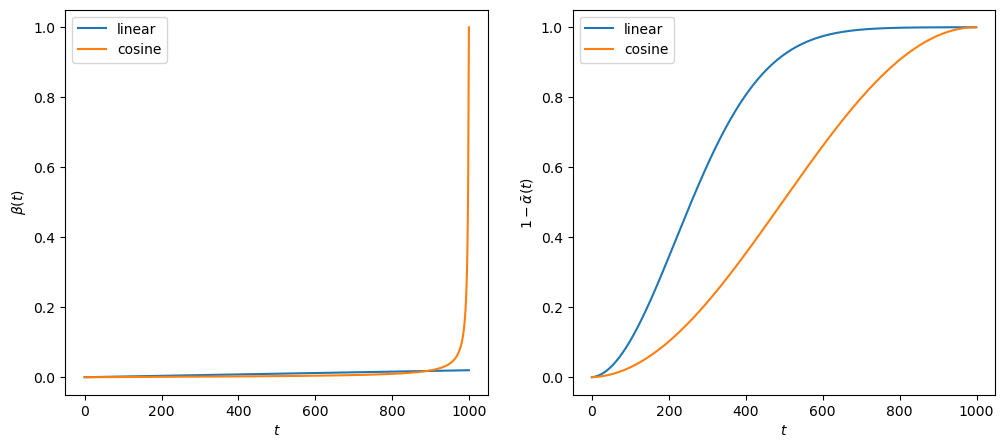
\includegraphics[width=.7\textwidth]{images/variance_schedule_alphadash.png}
    \caption{Variance Schedule Approaches: Modeling the $1-\bar{\alpha}$ as an approximate linear function (right cosine) and deriving $\beta$ (left cosine), or modeling $\beta$ as a linear function (left linear) and deriving $1-\bar{\alpha}$.}
    \label{fig:alphadash}
\end{figure}

The intution can experimentally confirmed by measuring how closely we get to isotropic noise when passing samples through the forward process. For this a batch of 50 times the same image was passed through the different steps of the process and the covariance matrix was calculated. As a metric for how close the covariance matrix was to the identity covariance matrix of pure i.i.d Gaussian noise, the identity matrix was subtracted and the mean of the absolute value of the matrix calculated. The results can be seen in Fig.~\ref{fig:noisecloseness} and confirm the intuition: When using linear scheduling we reach the closest point to pure noise already after around 600 steps for small images, and after around 700 for larger images. Cosine scheduling also performs worse on smaller images than on larger ones, but is still capable providing value for at least 850 timesteps.

\begin{figure}[h]
    \centering
    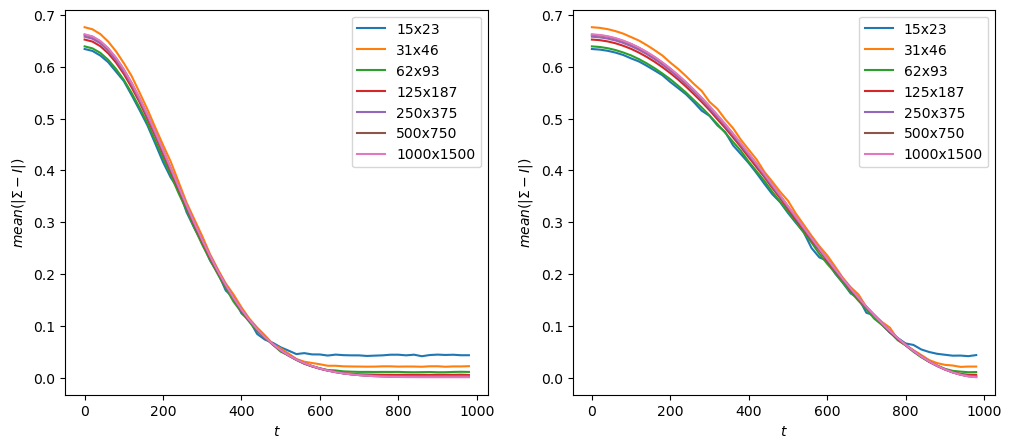
\includegraphics[width=.7\textwidth]{images/frobenius_norm.png}
    \caption{Closeness to noise for linear scheduling (left) and cosine scheduling (right).}
    \label{fig:noisecloseness}
\end{figure}